% Section content template for individual Educative lessons
% This file contains the actual content for a specific section
% Generated from Educative API section content

% Section: Enable Fault Tolerance and Failure Detection
% Section ID: 5842597234343936
% Section Slug: enable-fault-tolerance-and-failure-detection
% Generated: 2025-12-06T22:45:31.666387

\subsection{Handle temporary failures}\label{K38mqSxm09MZ3qi74yn0v}
\\
Typically, distributed systems use a quorum-based approach to handle failures. A quorum is the minimum number of votes required for a distributed transaction to proceed with an operation. If a server is part of the consensus and is down, then we can't perform the required operation. It affects the availability and durability of our system.\\
\strut \\
We'll use a sloppy quorum instead of strict quorum membership. Usually , a leader manages the communication among the participants of the consensus. The participants send an acknowledgment after committing a successful write. Upon receiving these acknowledgments, the leader responds to the client. However, the drawback is that the participants are easily affected by the network outage. If the leader is temporarily down and the participants can't reach it, they declare the leader dead. Now
, a new leader has to be reelected. Such frequent elections have a negative impact on performance because the system spends more time picking a leader than accomplishing any actual work.\\
\strut \\
In the sloppy quorum, the first \protect\phantomsection\label{katex_inline_SN8BXXhIbE11uPam6aHTL}{{{\(\text{n}\)}}} healthy nodes from the preference list handle all read and write operations. The
\protect\phantomsection\label{katex_inline_e49pm5MAdBHXfWYCkZgFR}{{{\(\text{n}\)}}} healthy nodes may not always be the first \protect\phantomsection\label{katex_inline_1pIhHCmbqN2TWwCufoJl4}{{{\(\text{n}\)}}} nodes discovered when moving clockwise in the consistent hash ring.\\
\strut \\
Let's consider the following configuration with \protect\phantomsection\label{katex_inline_w7i1ScJV9b-cOPvdVPf78}{{{\(\text{n = 3}\)}}}. If node \protect\phantomsection\label{katex_inline_j_S6kObcNFPD1oKeOBmLg}{{{\(\text{A}\)}}} is briefly unavailable or unreachable during a write operation, the request is sent to the next healthy node from the preference list, which is node \protect\phantomsection\label{katex_inline_b1o91B_iTFoEKKWtVOlzk}{{{\(\text{D}\)}}} in this case. It ensures the desired availability and durability. After processing the request, the node \protect\phantomsection\label{katex_inline_xPdkFH3ej_9CqB5TSVY9v}{{{\(\text{D}\)}}} includes a hint as to which node was the intended receiver (in this case, \protect\phantomsection\label{katex_inline_PCzK5y5PavbK9NYi1whtX}{{{\(\text{A}\)}}}). Once node \protect\phantomsection\label{katex_inline_uej8zMPTb-mgiAovQKkVk}{{{\(\text{A}\)}}} is up and running again, node \protect\phantomsection\label{katex_inline_i9yuwDqssmme1qOy518QD}{{{\(\text{D}\)}}} sends the request information to \protect\phantomsection\label{katex_inline_pr6xtPfJlo5D2V3X36edr}{{{\(\text{A}\)}}} so it can update its data. Upon completion of the transfer, \protect\phantomsection\label{katex_inline_WKIzD9HWCAnJIB9pBjqNk}{{{\(\text{D}\)}}} removes this item from its local storage without affecting the total number of replicas in the system.

\begin{figure}[htbp]
 \centering
 \begin{subfigure}[b]{0.48\textwidth}
 \centering
 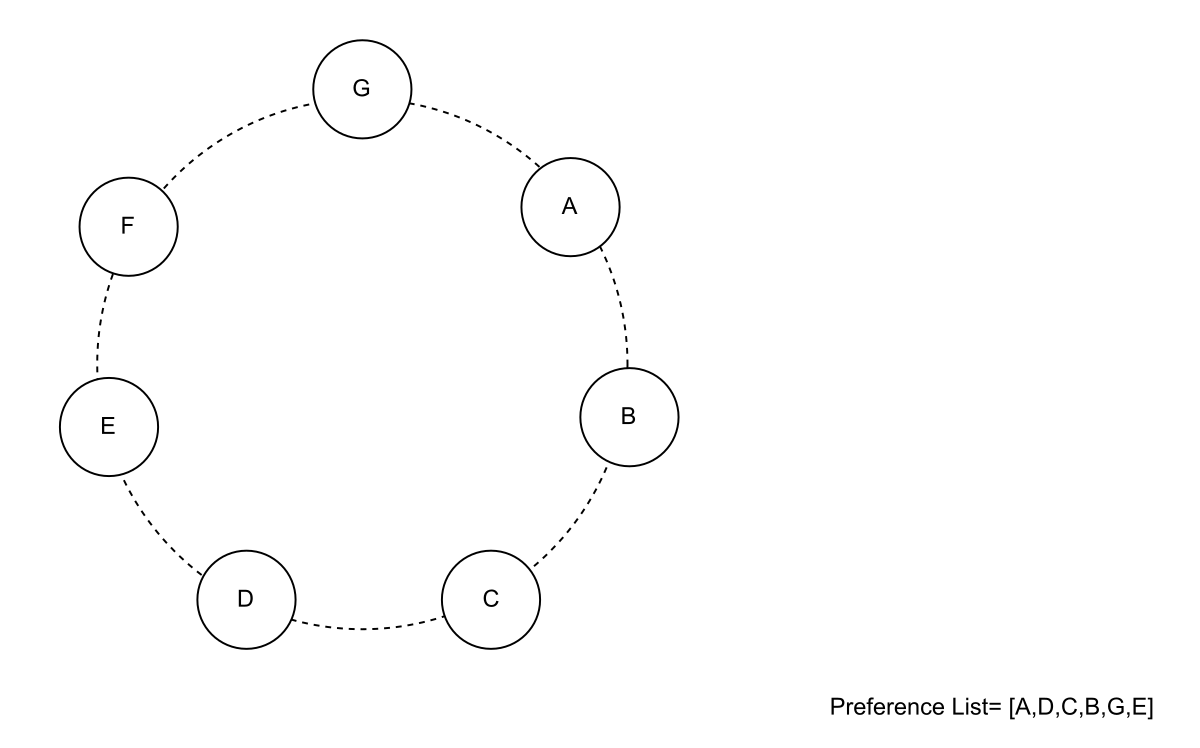
\includegraphics[width=\textwidth]{Images/chapter_10/section_5842597234343936/6026053982355456.png}
 \caption{Suppose we have seven nodes in our ring and a preference list of the nodes}
 \end{subfigure}
 \hfill
 \begin{subfigure}[b]{0.48\textwidth}
 \centering
 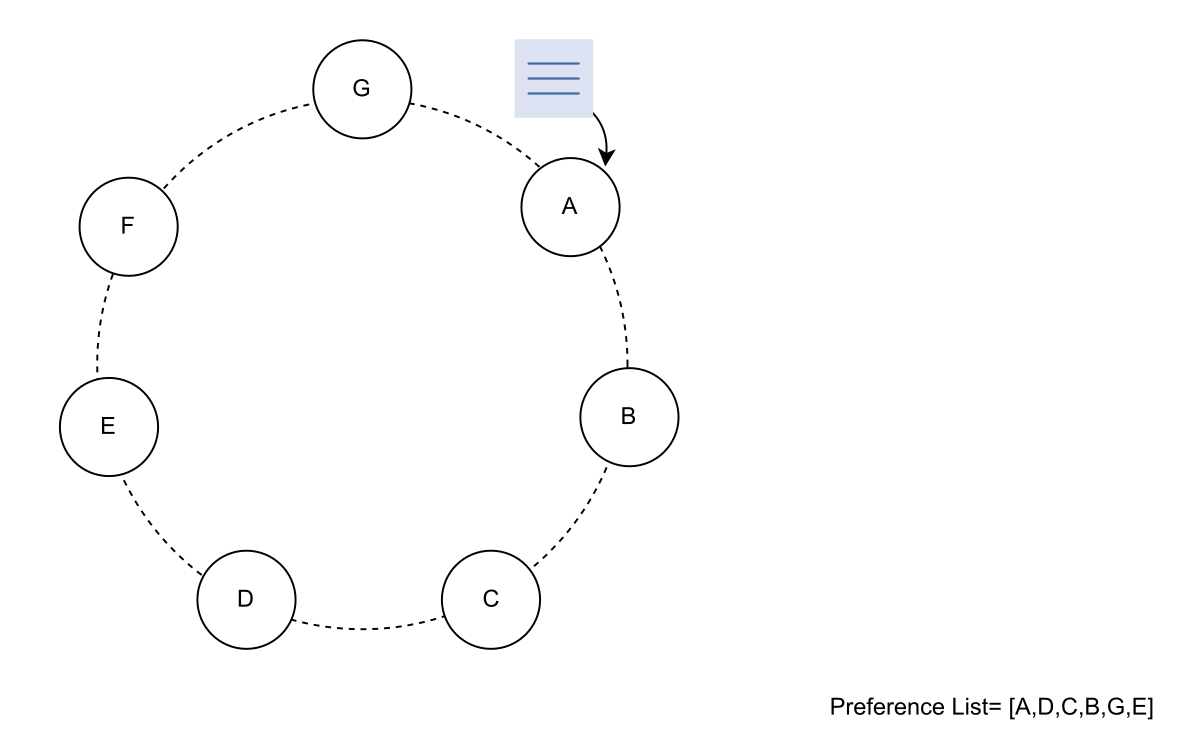
\includegraphics[width=\textwidth]{Images/chapter_10/section_5842597234343936/6571628872073216.png}
 \caption{A request comes in, and node A processes it since it’s the next node in the ring. The node is processed while moving in the clockwise direction}
 \end{subfigure}
\end{figure}

\begin{figure}[htbp]
 \centering
 \begin{subfigure}[b]{0.48\textwidth}
 \centering
 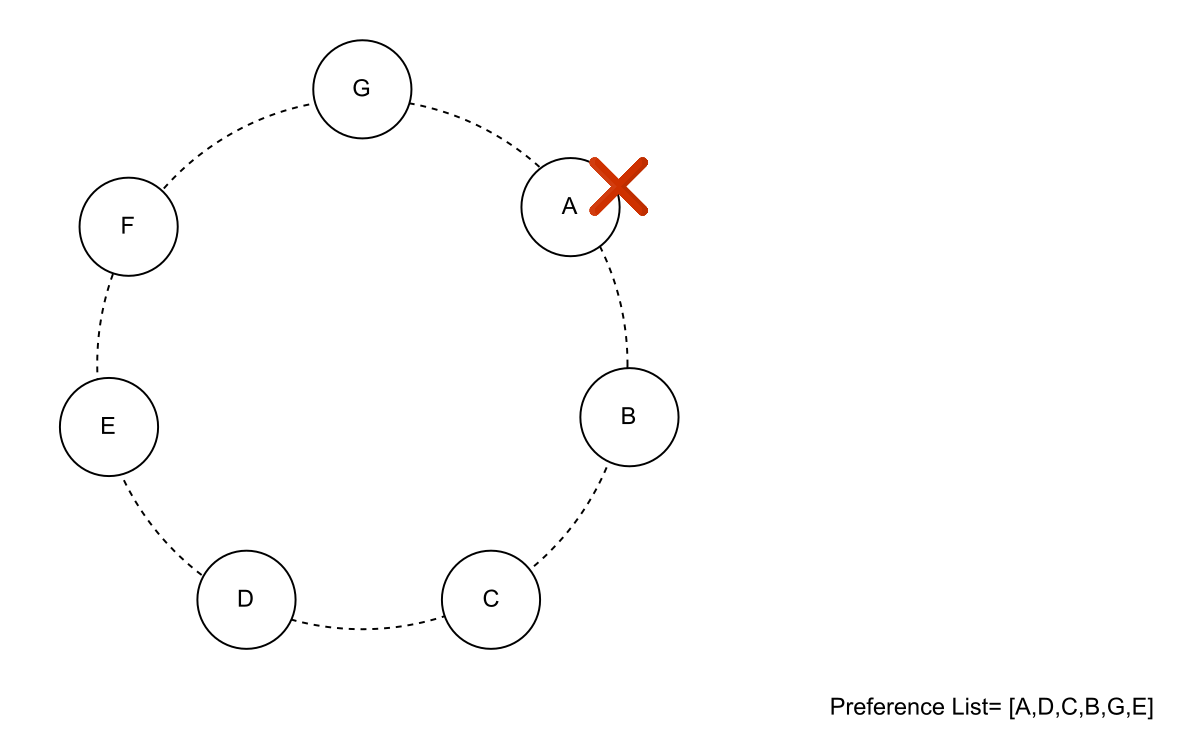
\includegraphics[width=\textwidth]{Images/chapter_10/section_5842597234343936/4899582534483968.png}
 \caption{Node A becomes down due to some failure}
 \end{subfigure}
 \hfill
 \begin{subfigure}[b]{0.48\textwidth}
 \centering
 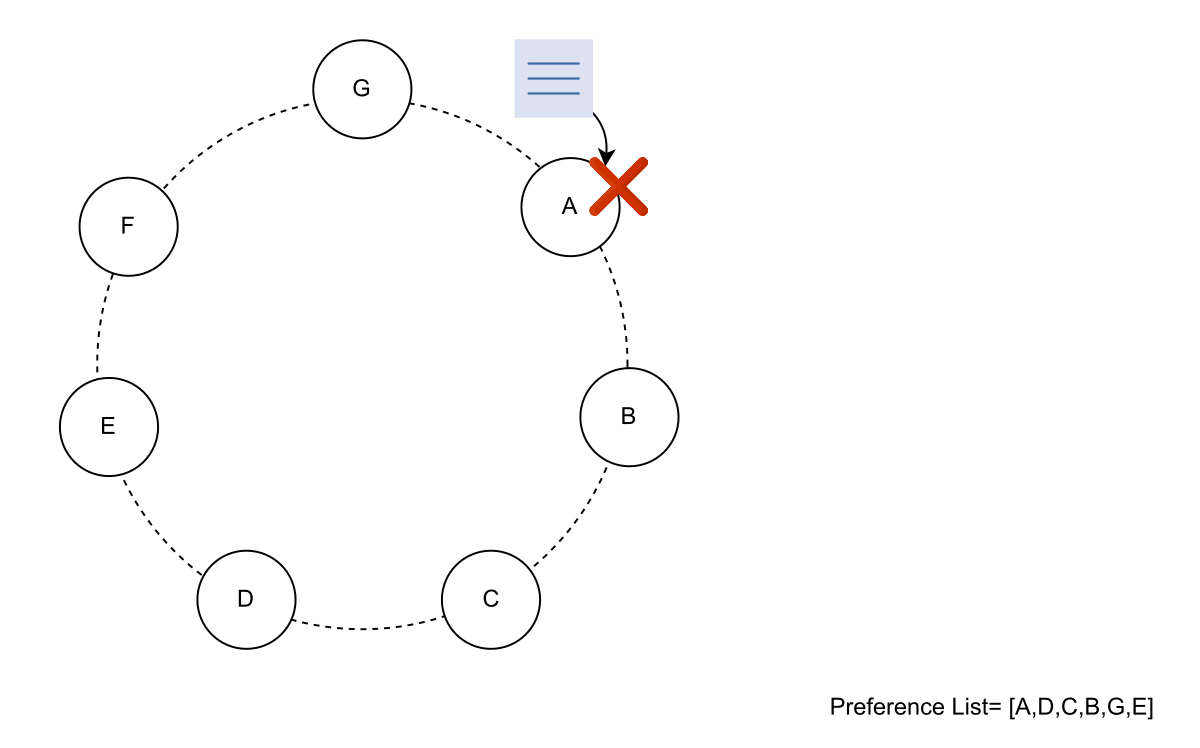
\includegraphics[width=\textwidth]{Images/chapter_10/section_5842597234343936/6388117737308160.png}
 \caption{A request comes in. Node A has to process it but is unable to, so we check the next node in the preference list}
 \end{subfigure}
\end{figure}

\begin{figure}[htbp]
 \centering
 \begin{subfigure}[b]{0.48\textwidth}
 \centering
 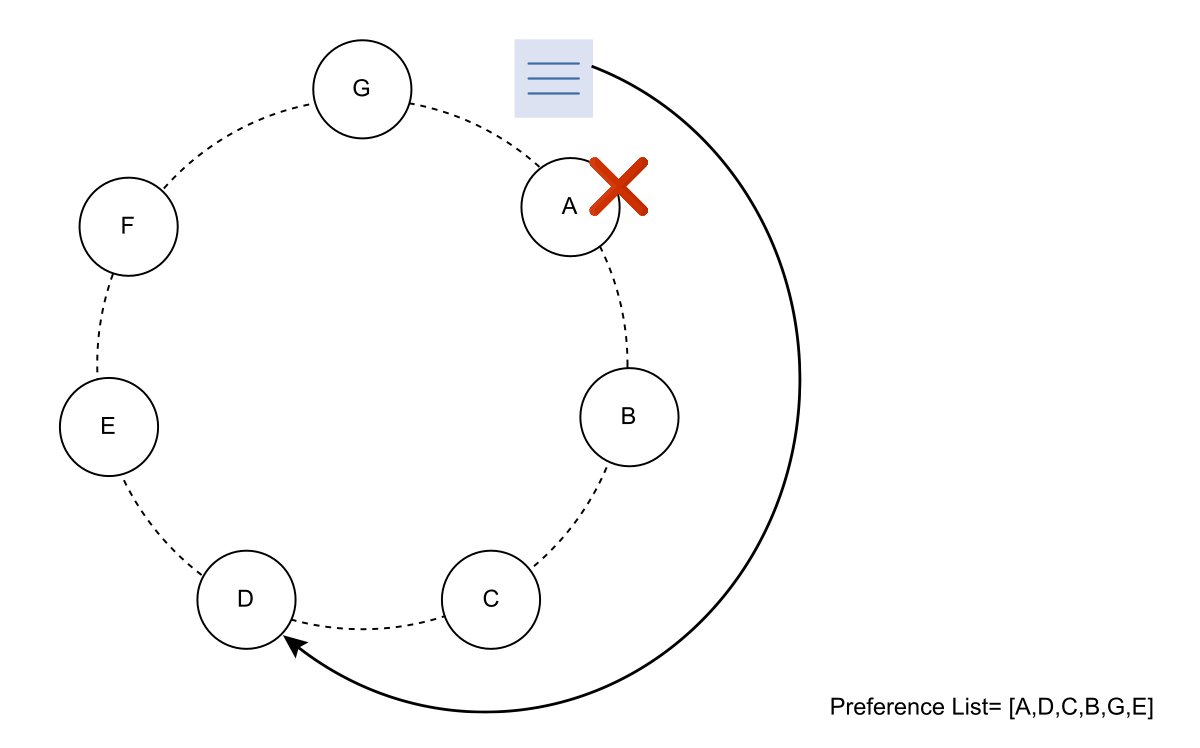
\includegraphics[width=\textwidth]{Images/chapter_10/section_5842597234343936/6200880986849280.png}
 \caption{Request is sent to node D as node A is down}
 \end{subfigure}
\end{figure}

This approach is called a \textbf{hinted handoff}. Using it, we can ensure that reads and writes are fulfilled if a node faces temporary failure.
\begin{quote}
\textbf{Note}: A highly available storage system must handle data center failure due to power outages, cooling failures, network failures, or natural disasters. For this, we should ensure replication across the data centers. So, if one data center is down, we can recover it from the other.
\end{quote}
\\
Hinted handoff helps maintain availability when nodes fail temporarily. But what happens when the system experiences prolonged failures?

\textbf{Question:}

The limitations of hinted handoff

\textbf{Reference Answer:}

When a node remains down beyond the hinted handoff window, those temporary hints expire or are discarded to prevent unbounded storage growth. At that point, the system shifts from fast recovery to full data reconciliation. Once the node returns, background processes like anti-entropy repair, read repair, or Merkle tree comparison detect and synchronize missing updates, potentially at the cost of temporary inconsistency or data loss if recovery is delayed too long.

\subsection{Handle permanent failures}\label{anzKzvAjpnqSPjLjcBA4F}
\\
In the event of permanent failures of nodes, we should keep our replicas synchronized to make our system more durable. We need to speed up the detection of inconsistencies between replicas and reduce the quantity of transferred data. We 'll use Merkle trees for that.
\\
In a \textbf{Merkle tree}, the values of individual keys are hashed and used as the leaves of the tree. There are hashes of their children in the parent nodes higher up the tree. Each branch of the Merkle tree can be verified independently without the need to download the complete tree or the entire dataset. While checking for inconsistencies across copies, Merkle trees reduce the amount of data that must be exchanged. There's no need for synchronization if, for example, the hash values of two trees' roots are the same and their leaf nodes are also the same. Until the process reaches the tree leaves, the hosts can identify the keys that are out of sync when the nodes exchange the hash values of children. The Merkle tree is a mechanism to implement anti-entropy, which means to keep all the data consistent. It reduces data transmission for synchronization and the number of discs accessed during the anti-entropy process.
\\
The following slides explain how Merkle trees work:

\begin{figure}[htbp]
 \centering
 \begin{subfigure}[b]{0.48\textwidth}
 \centering
 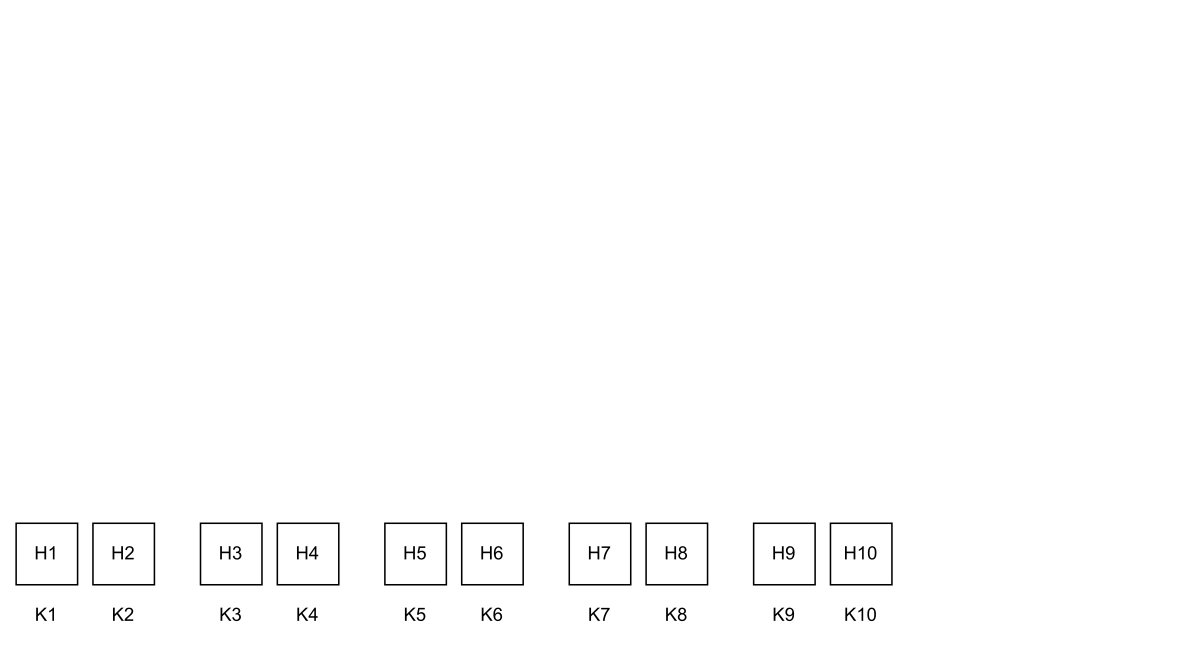
\includegraphics[width=\textwidth]{Images/chapter_10/section_5842597234343936/4894607284633600.png}
 \caption{Calculate the hashes for all keys. The hashes will be leaf nodes}
 \end{subfigure}
 \hfill
 \begin{subfigure}[b]{0.48\textwidth}
 \centering
 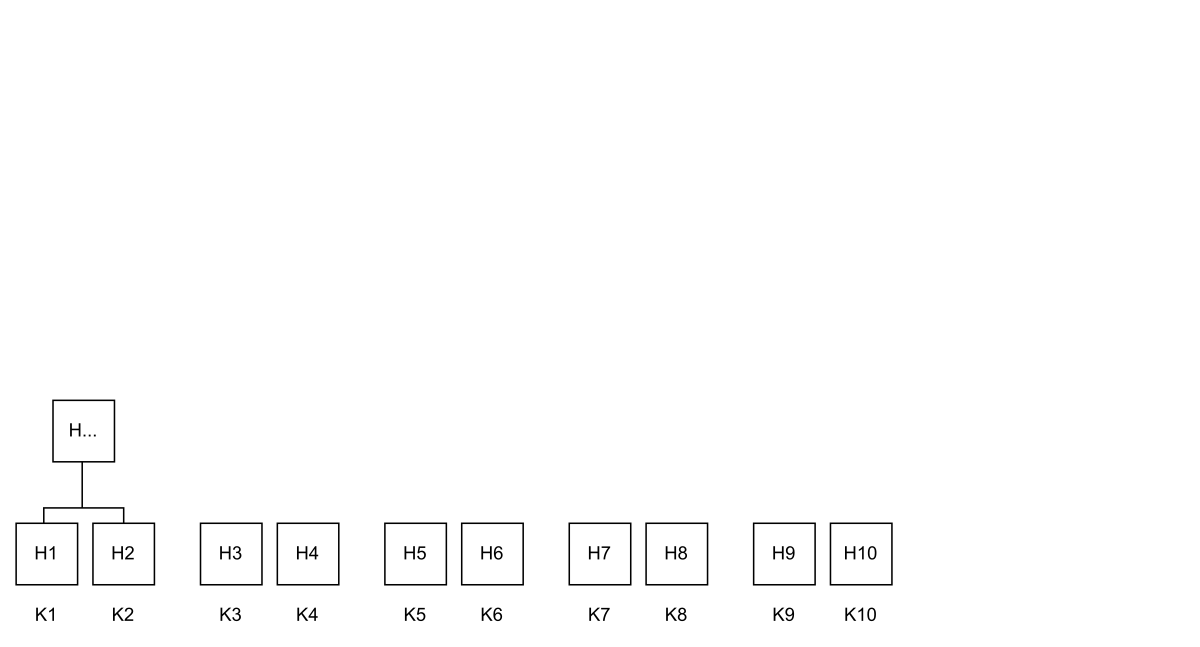
\includegraphics[width=\textwidth]{Images/chapter_10/section_5842597234343936/6656784182018048.png}
 \caption{The hashes of the H1 and H2 nodes are calculated and stored as their parent node}
 \end{subfigure}
\end{figure}

\begin{figure}[htbp]
 \centering
 \begin{subfigure}[b]{0.48\textwidth}
 \centering
 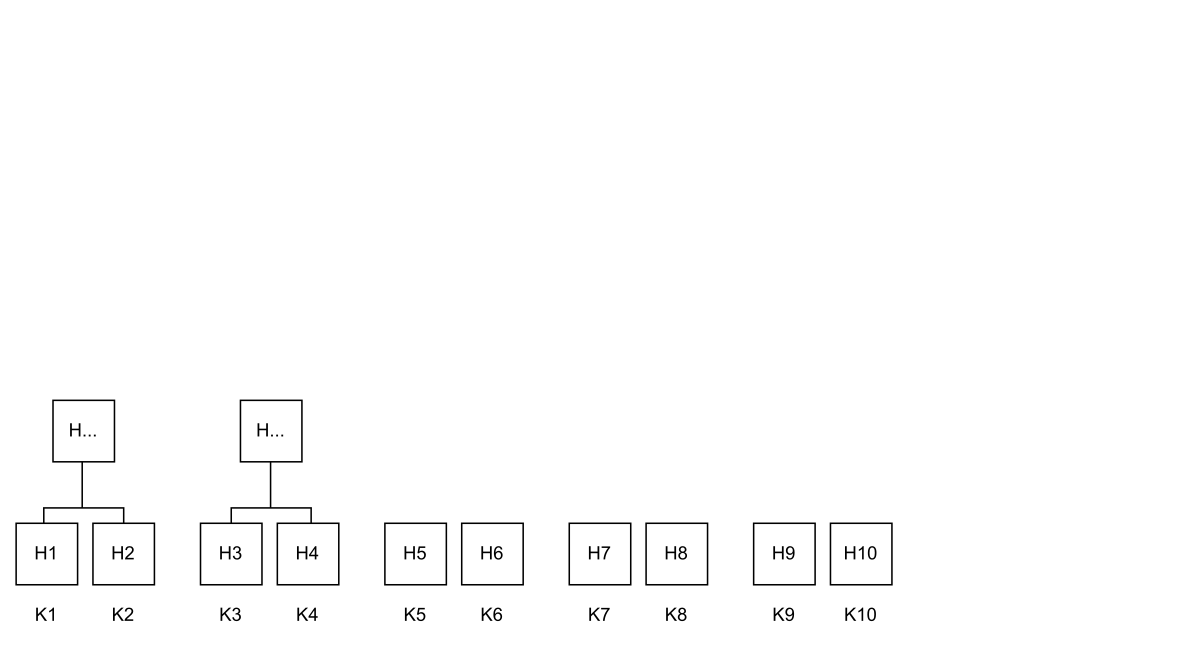
\includegraphics[width=\textwidth]{Images/chapter_10/section_5842597234343936/4746170866073600.png}
 \caption{The hashes of the H3 and H4 nodes are calculated and stored as their parent node}
 \end{subfigure}
 \hfill
 \begin{subfigure}[b]{0.48\textwidth}
 \centering
 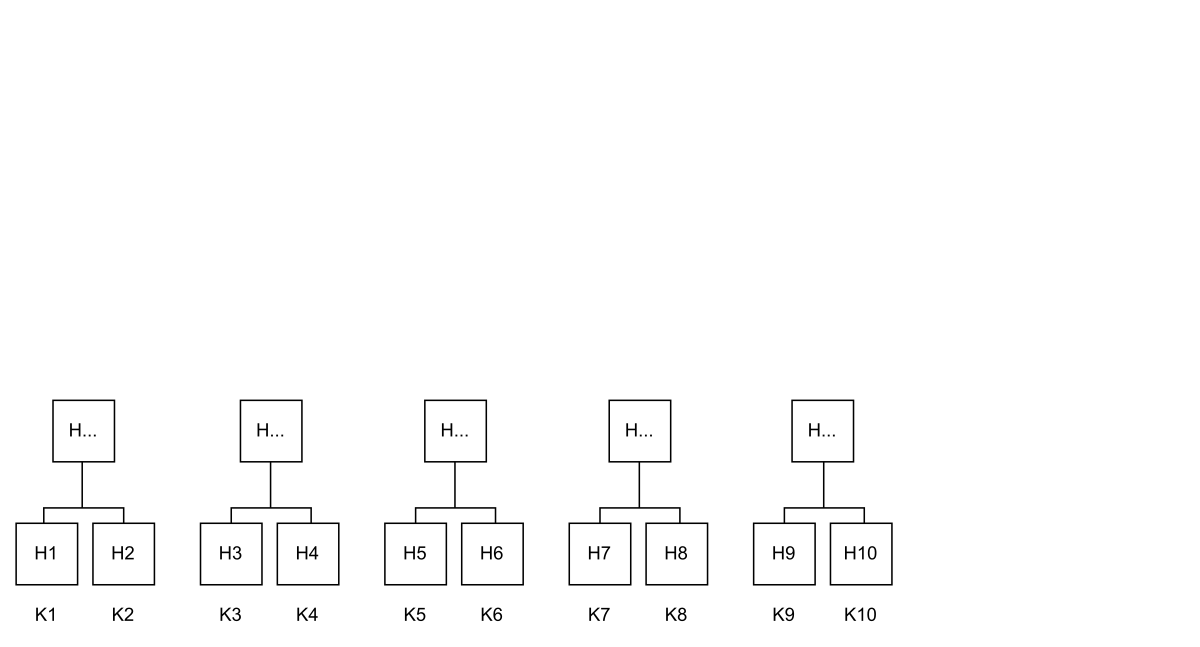
\includegraphics[width=\textwidth]{Images/chapter_10/section_5842597234343936/6143611892924416.png}
 \caption{The hashes of all other nodes are calculated and stored as their parent node}
 \end{subfigure}
\end{figure}

\begin{figure}[htbp]
 \centering
 \begin{subfigure}[b]{0.48\textwidth}
 \centering
 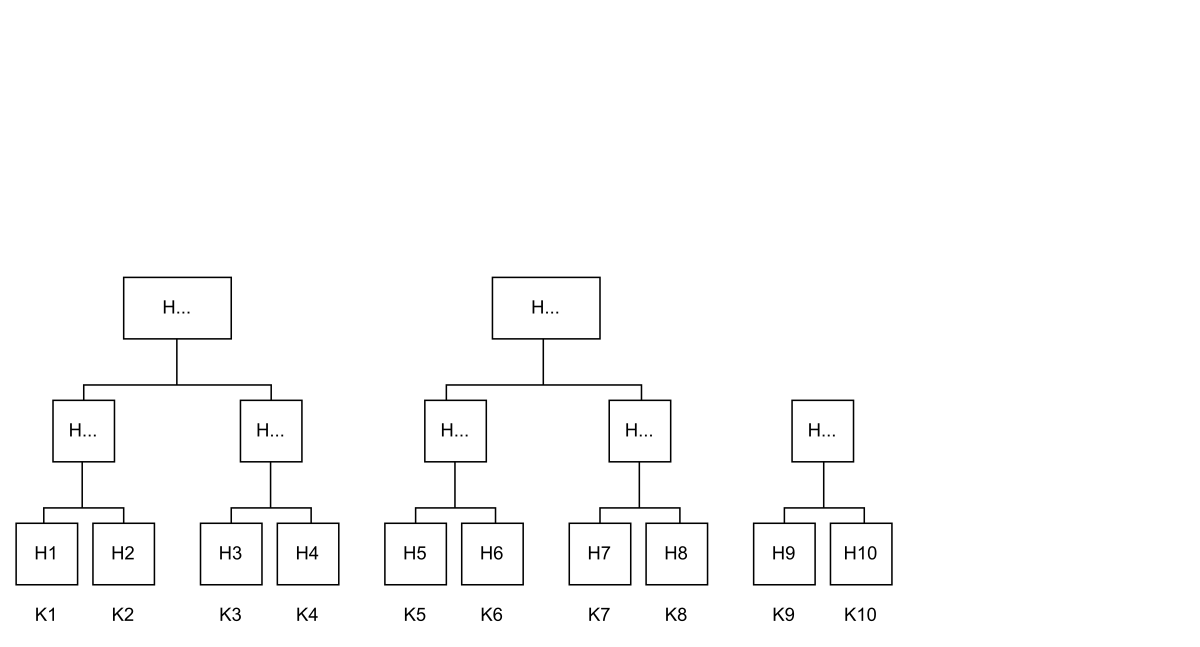
\includegraphics[width=\textwidth]{Images/chapter_10/section_5842597234343936/4646777873760256.png}
 \caption{The hashes of the nodes H 1 2 and H 3 4 is calculated and stored as their parent node. The same thing is done for H 5 6 and H 7 8}
 \end{subfigure}
 \hfill
 \begin{subfigure}[b]{0.48\textwidth}
 \centering
 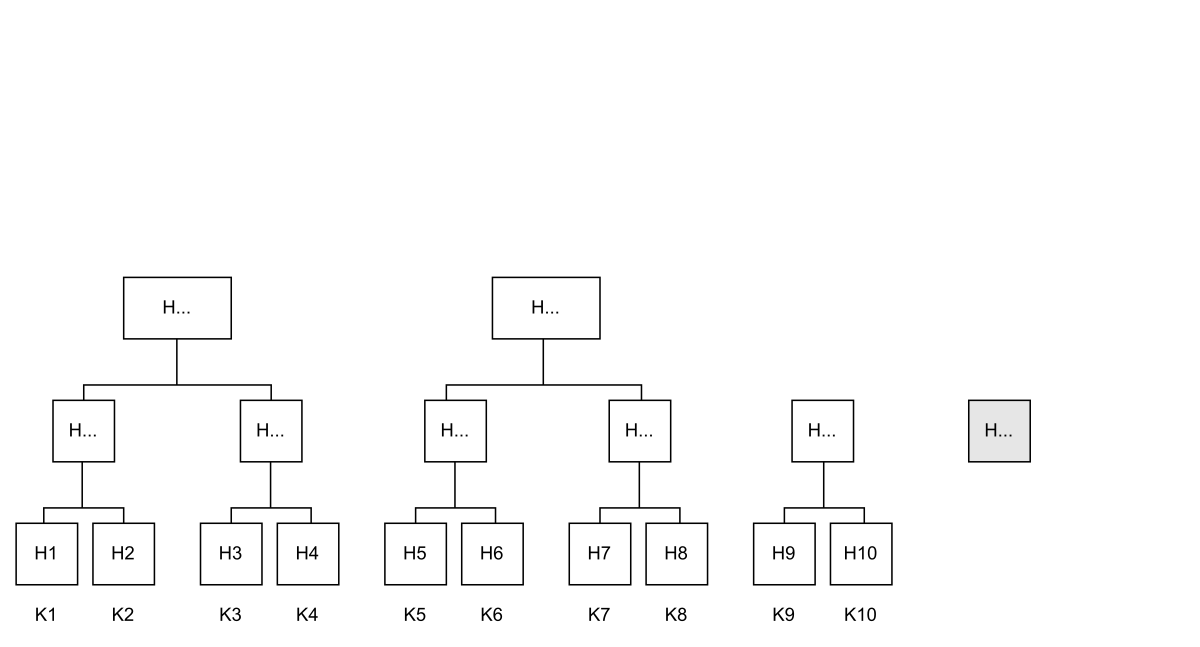
\includegraphics[width=\textwidth]{Images/chapter_10/section_5842597234343936/5553562440695808.png}
 \caption{We duplicate the odd node}
 \end{subfigure}
\end{figure}

\begin{figure}[htbp]
 \centering
 \begin{subfigure}[b]{0.48\textwidth}
 \centering
 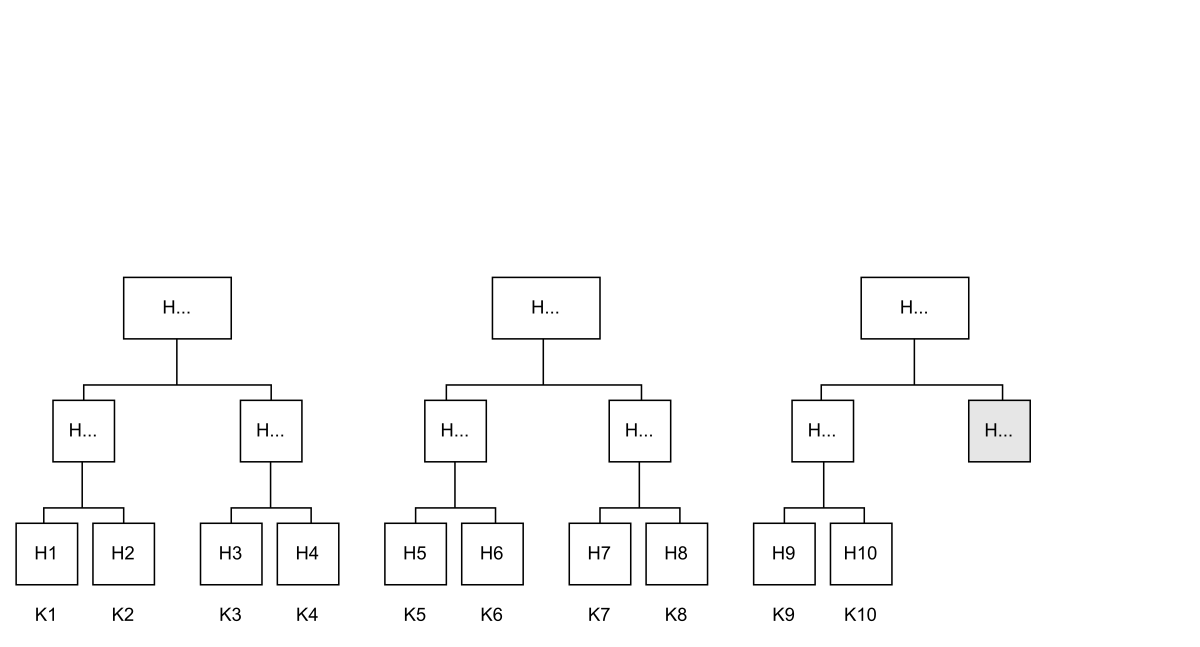
\includegraphics[width=\textwidth]{Images/chapter_10/section_5842597234343936/6585363816775680.png}
 \caption{Calculate the hash of both nodes (the actual node and its duplicate), and store it as the parent node}
 \end{subfigure}
 \hfill
 \begin{subfigure}[b]{0.48\textwidth}
 \centering
 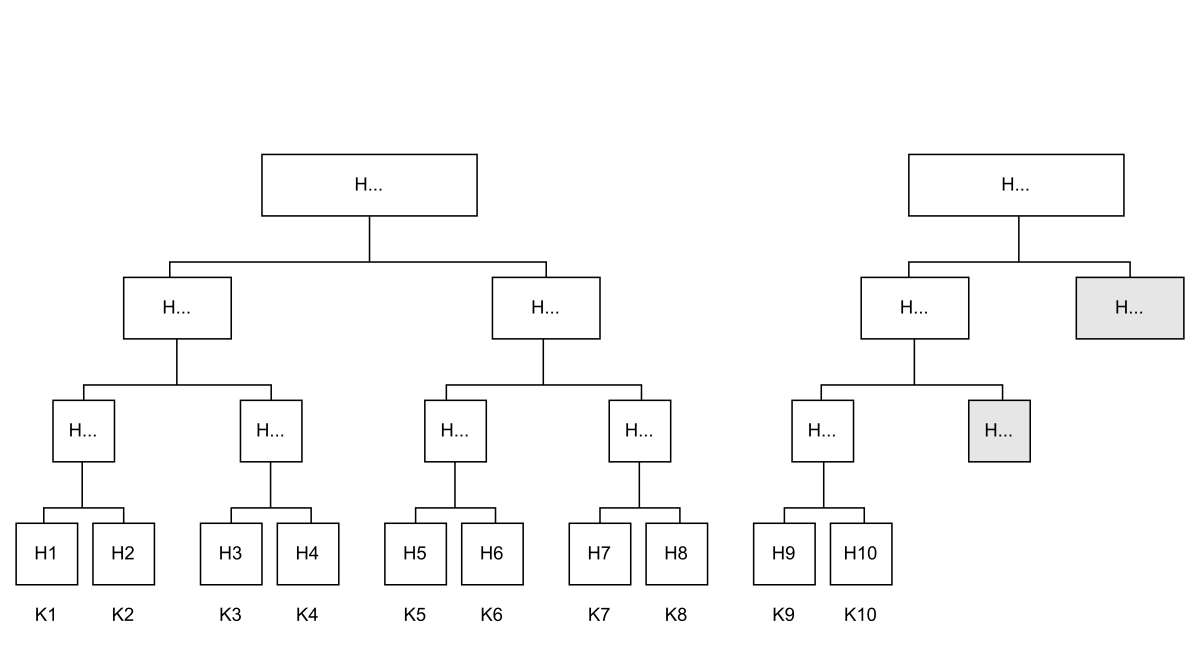
\includegraphics[width=\textwidth]{Images/chapter_10/section_5842597234343936/5467684770938880.png}
 \caption{Calculate the hash of the nodes and store them as the parent node}
 \end{subfigure}
\end{figure}

\begin{figure}[htbp]
 \centering
 \begin{subfigure}[b]{0.48\textwidth}
 \centering
 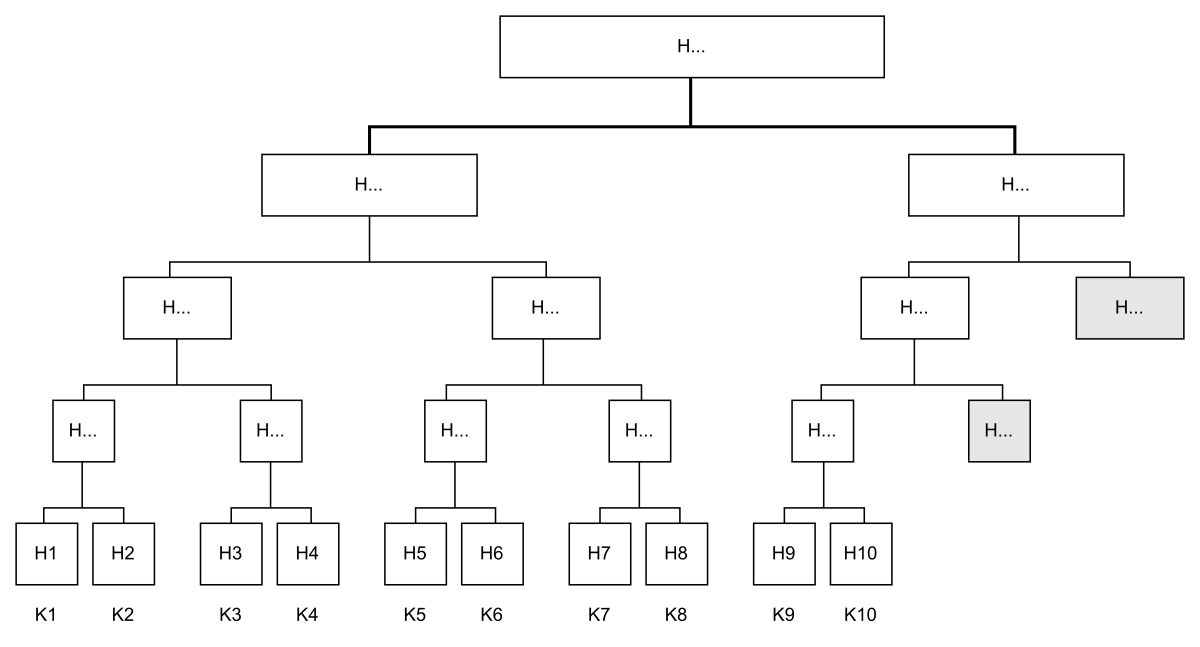
\includegraphics[width=\textwidth]{Images/chapter_10/section_5842597234343936/6630097780211712.png}
 \caption{Calculate the hash of the last two nodes to store as the root node}
 \end{subfigure}
 \hfill
 \begin{subfigure}[b]{0.48\textwidth}
 \centering
 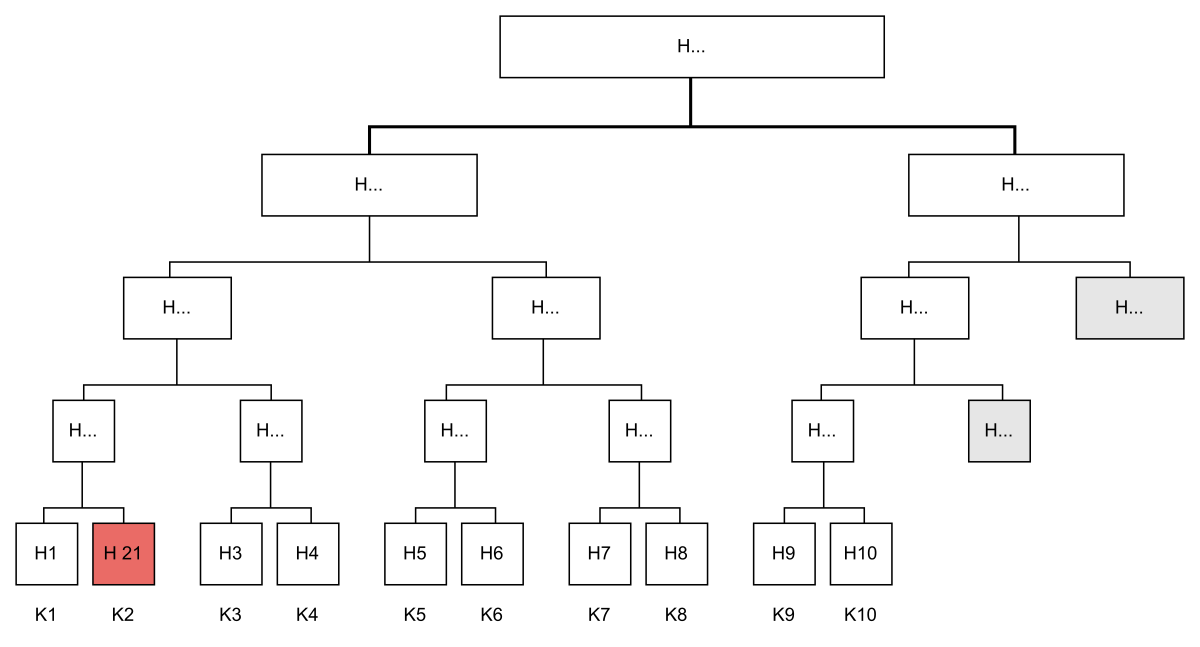
\includegraphics[width=\textwidth]{Images/chapter_10/section_5842597234343936/5200180316209152.png}
 \caption{Suppose the value of K2 is updated. Its hash will now be recalculated}
 \end{subfigure}
\end{figure}

\begin{figure}[htbp]
 \centering
 \begin{subfigure}[b]{0.48\textwidth}
 \centering
 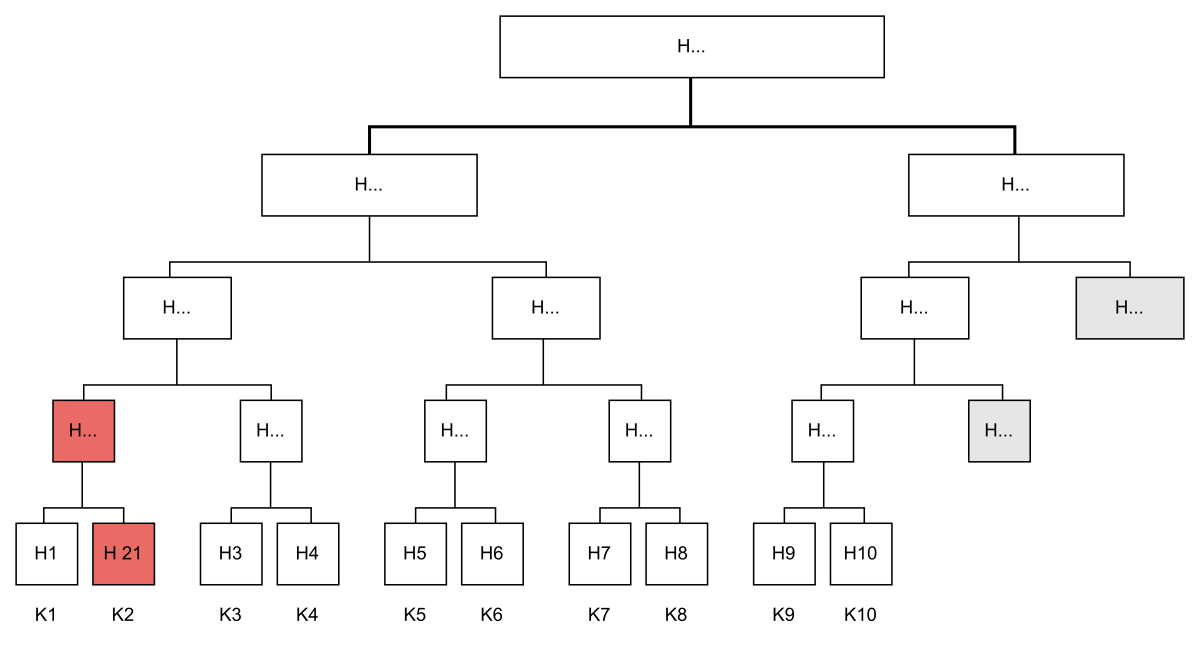
\includegraphics[width=\textwidth]{Images/chapter_10/section_5842597234343936/5553552441475072.png}
 \caption{The hash of the parent will also be recalculated and updated}
 \end{subfigure}
 \hfill
 \begin{subfigure}[b]{0.48\textwidth}
 \centering
 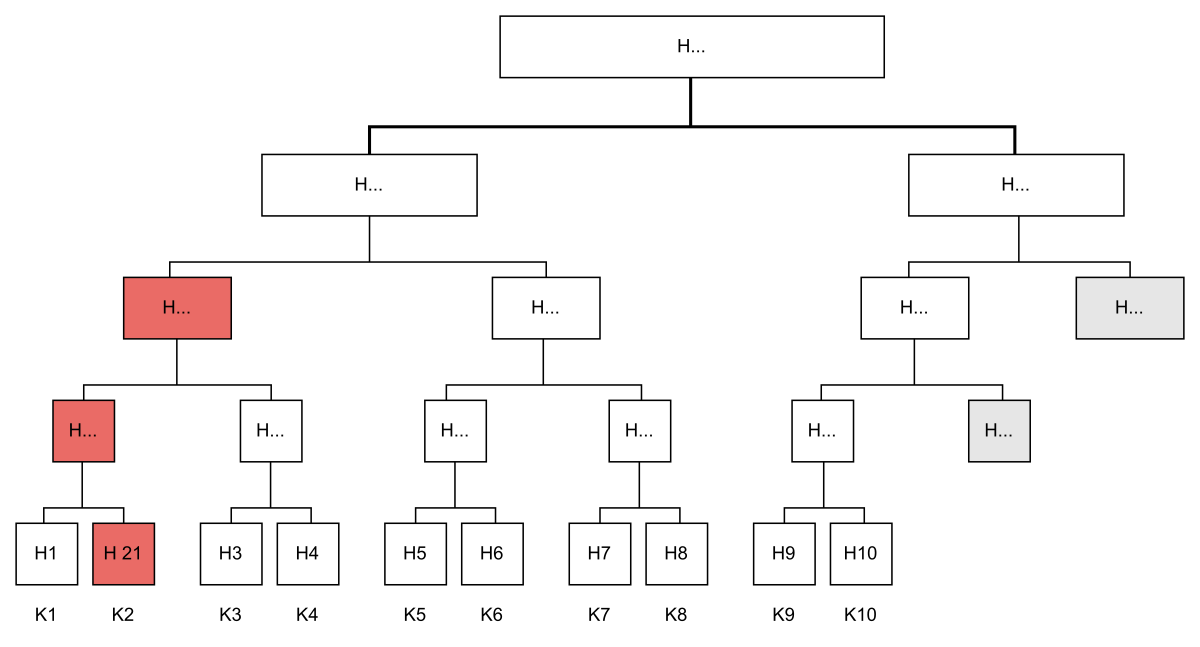
\includegraphics[width=\textwidth]{Images/chapter_10/section_5842597234343936/5187022079918080.png}
 \caption{The hash of the parent will also be recalculated and updated}
 \end{subfigure}
\end{figure}

\begin{figure}[htbp]
 \centering
 \begin{subfigure}[b]{0.48\textwidth}
 \centering
 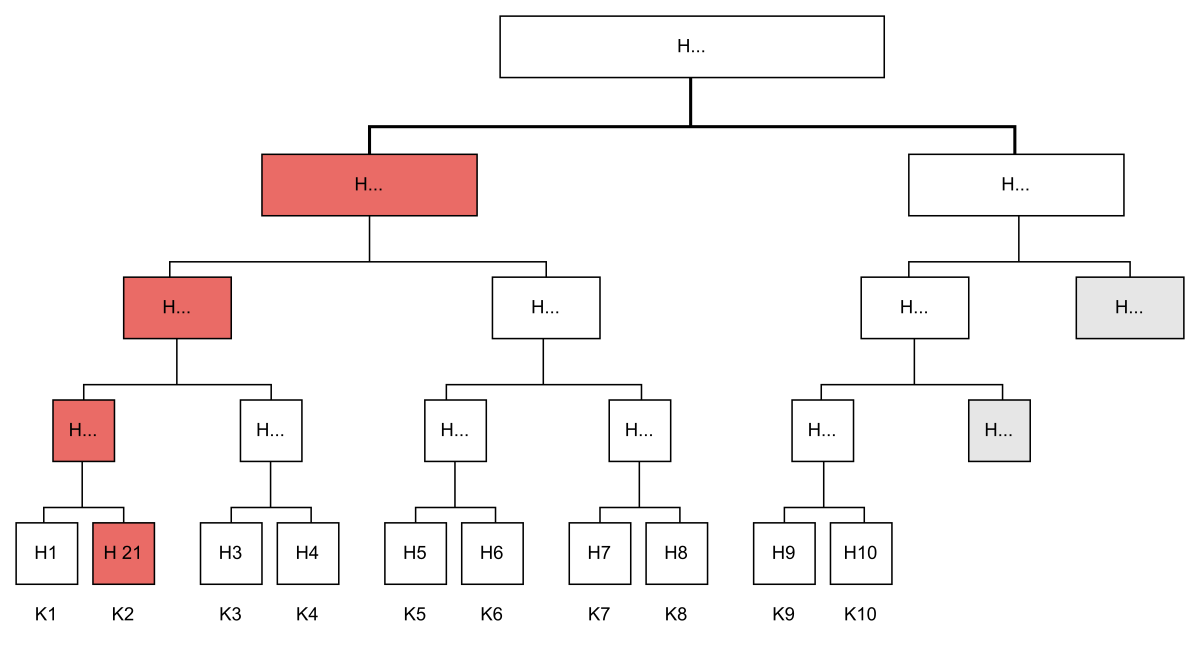
\includegraphics[width=\textwidth]{Images/chapter_10/section_5842597234343936/5532900158341120.png}
 \caption{The hash of the parent will also be recalculated and updated}
 \end{subfigure}
 \hfill
 \begin{subfigure}[b]{0.48\textwidth}
 \centering
 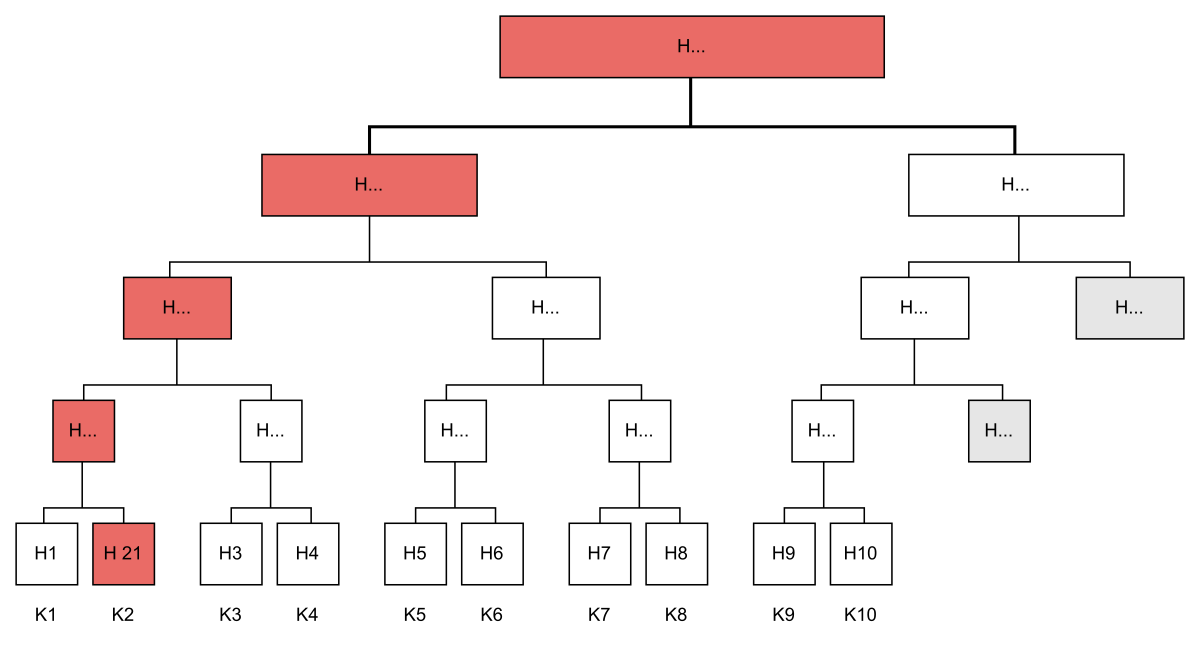
\includegraphics[width=\textwidth]{Images/chapter_10/section_5842597234343936/5999757734707200.png}
 \caption{The hash of the root node will also be recalculated and updated}
 \end{subfigure}
\end{figure}

\subsubsection{Anti-entropy with Merkle trees}\label{fIsSW0pd2bnn5am1e4LI2}
\\
Each node keeps a distinct Merkle tree for the range of keys that it hosts for each virtual node. The nodes can determine if the keys in a given range are correct. The root of the Merkle tree corresponding to the common key ranges is exchanged between two nodes. We 'll make the following comparison:

\begin{enumerate}
\item
\protect\phantomsection\label{eCiC0YufMUnjp1N5fhdAT}
Compare the hashes of the root node of Merkle trees.
\item
\protect\phantomsection\label{rjDRz0egrnyBIwoz7AU23}
Do not proceed if they're the same.
\item
\protect\phantomsection\label{yF3RhdzwmfmysTgRCRKtD}
Traverse left and right children using recursion. The nodes identify whether or not they have any differences and perform the necessary synchronization.
\end{enumerate}
\\
The following slides explain more about how Merkle trees work.
\begin{quote}
\textbf{Note}: We assume the ranges defined are hypothetical for illustration purposes.
\end{quote}

\begin{figure}[htbp]
 \centering
 \begin{subfigure}[b]{0.48\textwidth}
 \centering
 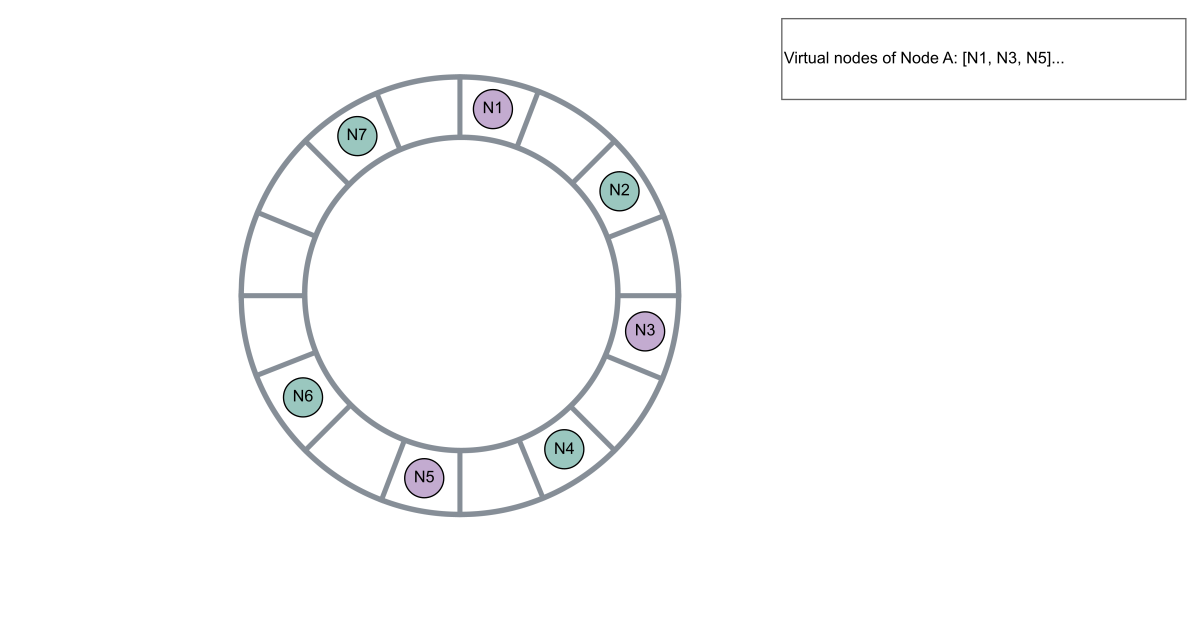
\includegraphics[width=\textwidth]{Images/chapter_10/section_5842597234343936/6334920666644480.png}
 \caption{Let’s suppose we have the virtual nodes A and B in the ring}
 \end{subfigure}
 \hfill
 \begin{subfigure}[b]{0.48\textwidth}
 \centering
 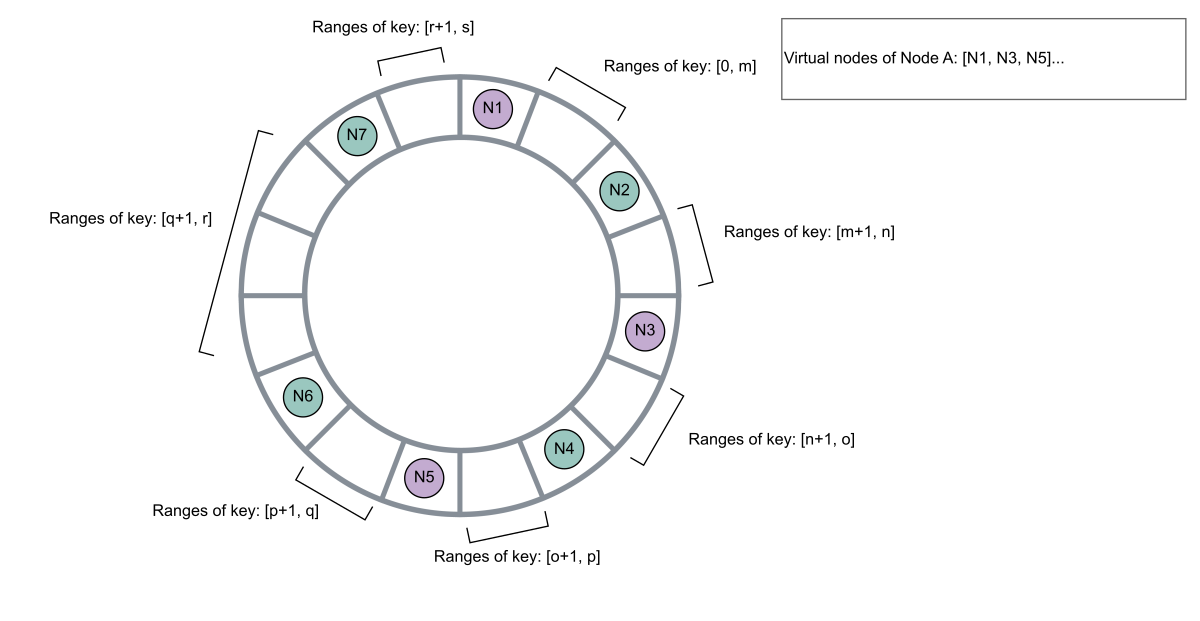
\includegraphics[width=\textwidth]{Images/chapter_10/section_5842597234343936/5164683409752064.png}
 \caption{The ranges that each virtual node covers are defined}
 \end{subfigure}
\end{figure}

\begin{figure}[htbp]
 \centering
 \begin{subfigure}[b]{0.48\textwidth}
 \centering
 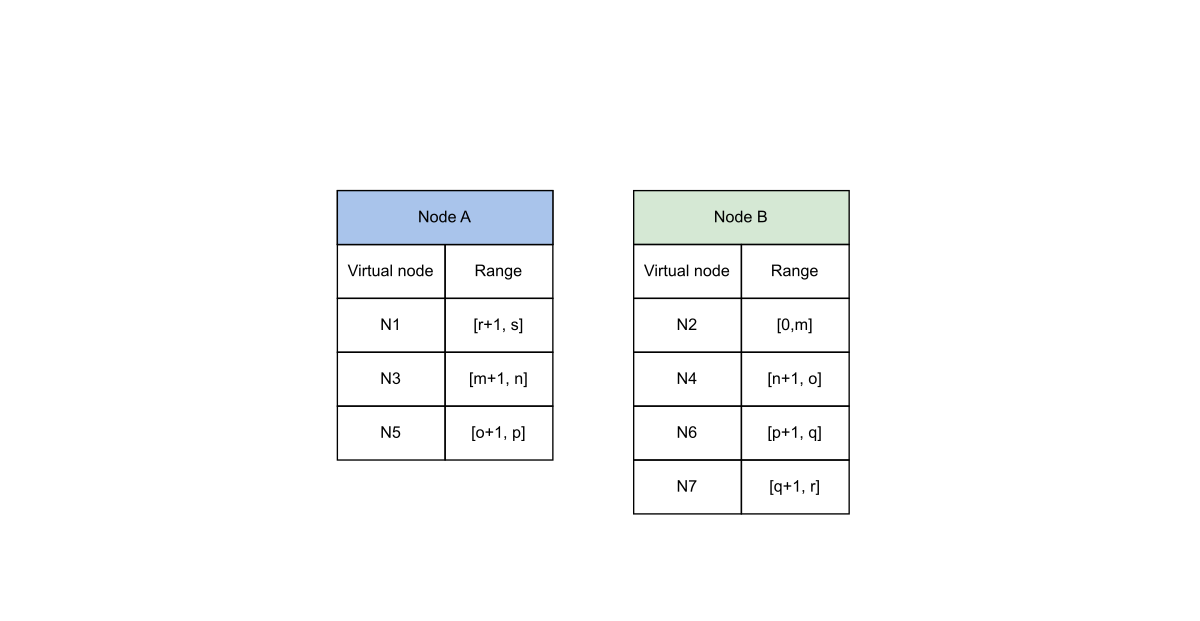
\includegraphics[width=\textwidth]{Images/chapter_10/section_5842597234343936/5344787762249728.png}
 \caption{The ranges that each virtual node covers are defined in table form}
 \end{subfigure}
 \hfill
 \begin{subfigure}[b]{0.48\textwidth}
 \centering
 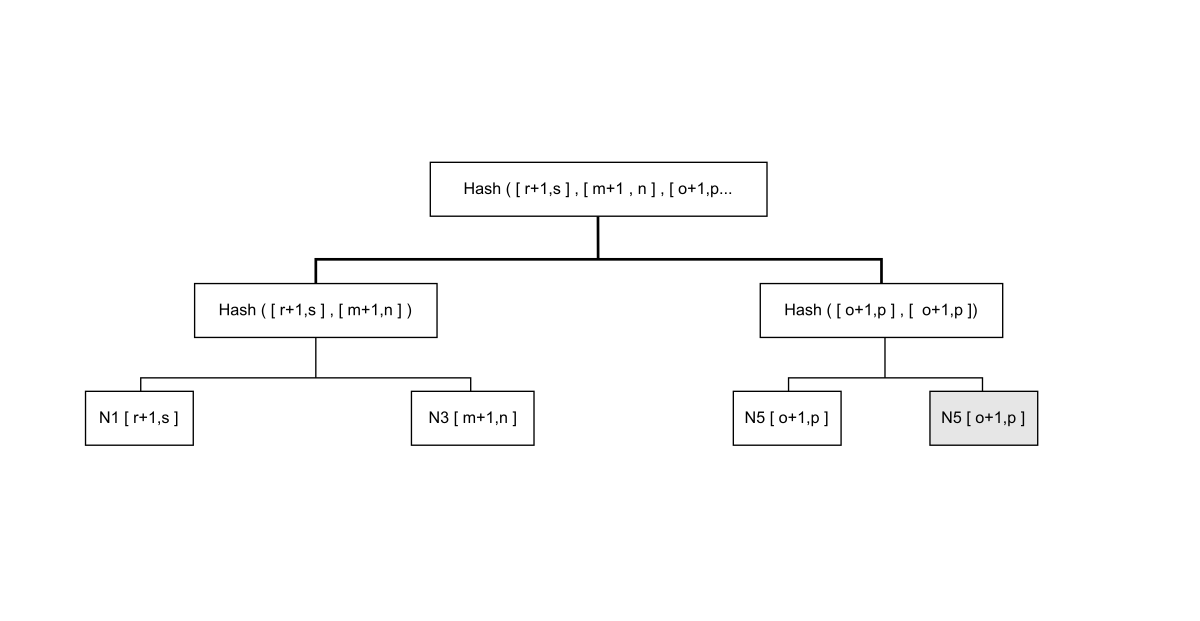
\includegraphics[width=\textwidth]{Images/chapter_10/section_5842597234343936/5515415346479104.png}
 \caption{Merkle tree for Node A}
 \end{subfigure}
\end{figure}

\begin{figure}[htbp]
 \centering
 \begin{subfigure}[b]{0.48\textwidth}
 \centering
 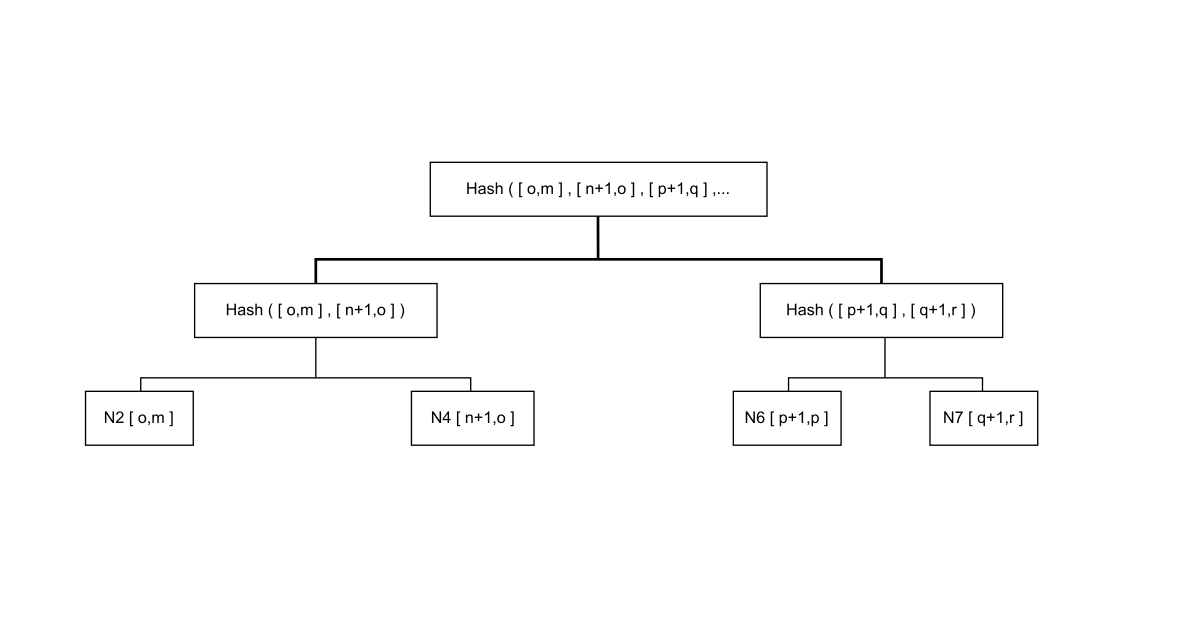
\includegraphics[width=\textwidth]{Images/chapter_10/section_5842597234343936/6284952622858240.png}
 \caption{Merkle tree for Node B}
 \end{subfigure}
 \hfill
 \begin{subfigure}[b]{0.48\textwidth}
 \centering
 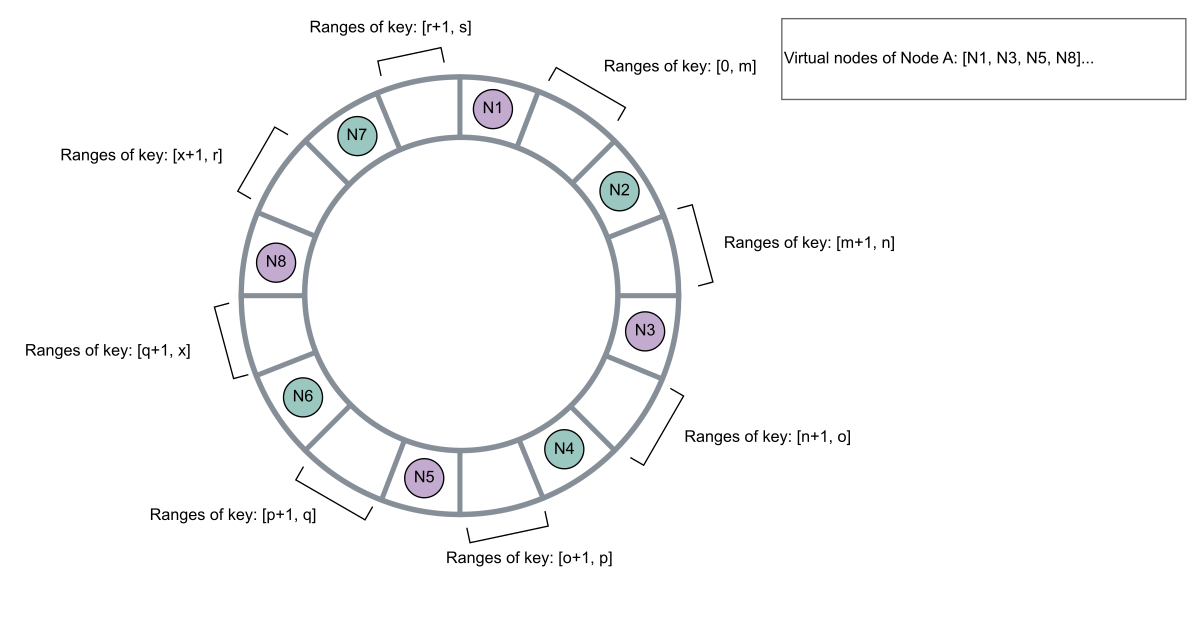
\includegraphics[width=\textwidth]{Images/chapter_10/section_5842597234343936/5471861483241472.png}
 \caption{Let’s suppose a new virtual node, N8, of A is added and the ranges are updated accordingly}
 \end{subfigure}
\end{figure}

\begin{figure}[htbp]
 \centering
 \begin{subfigure}[b]{0.48\textwidth}
 \centering
 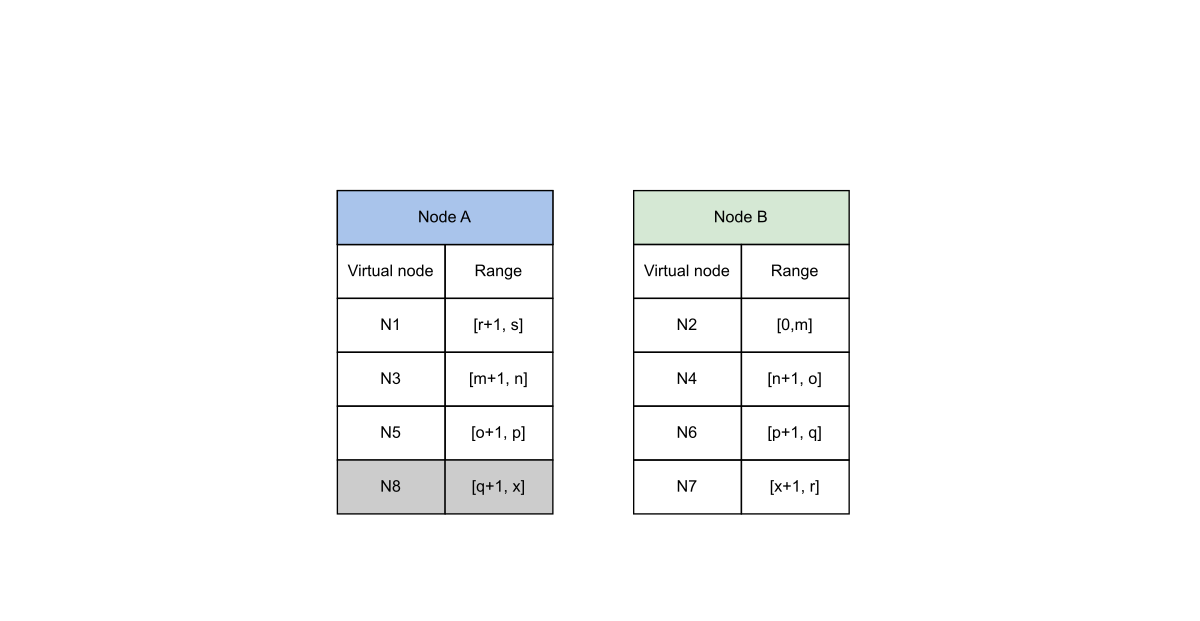
\includegraphics[width=\textwidth]{Images/chapter_10/section_5842597234343936/5517999499116544.png}
 \caption{The updated ranges that each virtual node covers are defined in table form}
 \end{subfigure}
 \hfill
 \begin{subfigure}[b]{0.48\textwidth}
 \centering
 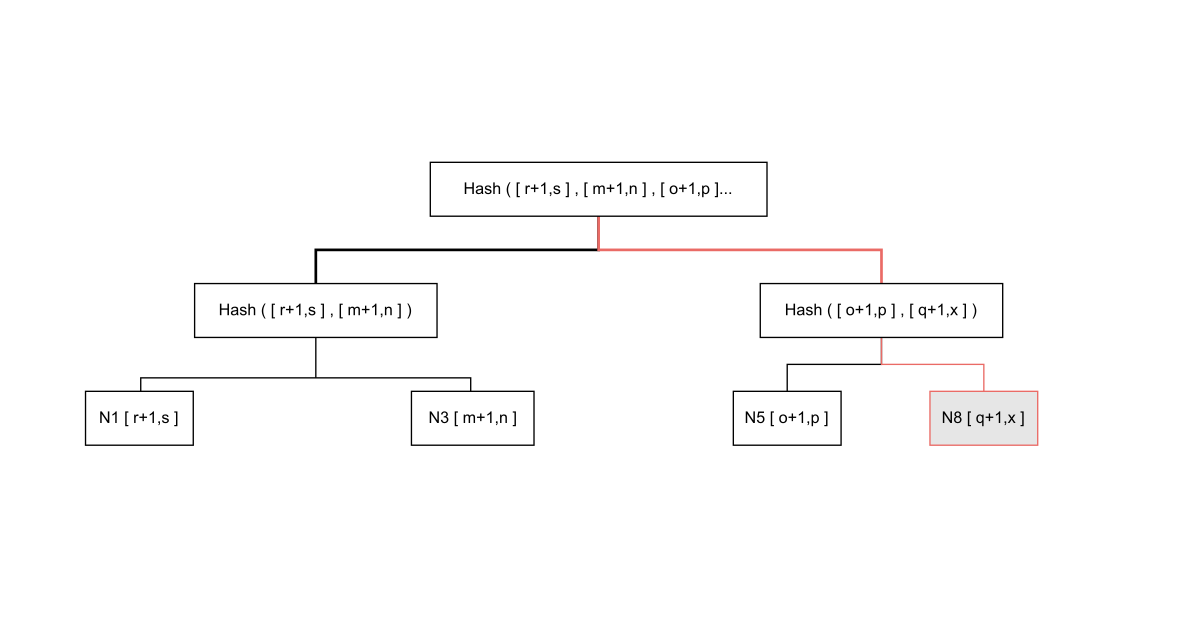
\includegraphics[width=\textwidth]{Images/chapter_10/section_5842597234343936/6292953912049664.png}
 \caption{The updated Merkle tree for Node A}
 \end{subfigure}
\end{figure}

\begin{figure}[htbp]
 \centering
 \begin{subfigure}[b]{0.48\textwidth}
 \centering
 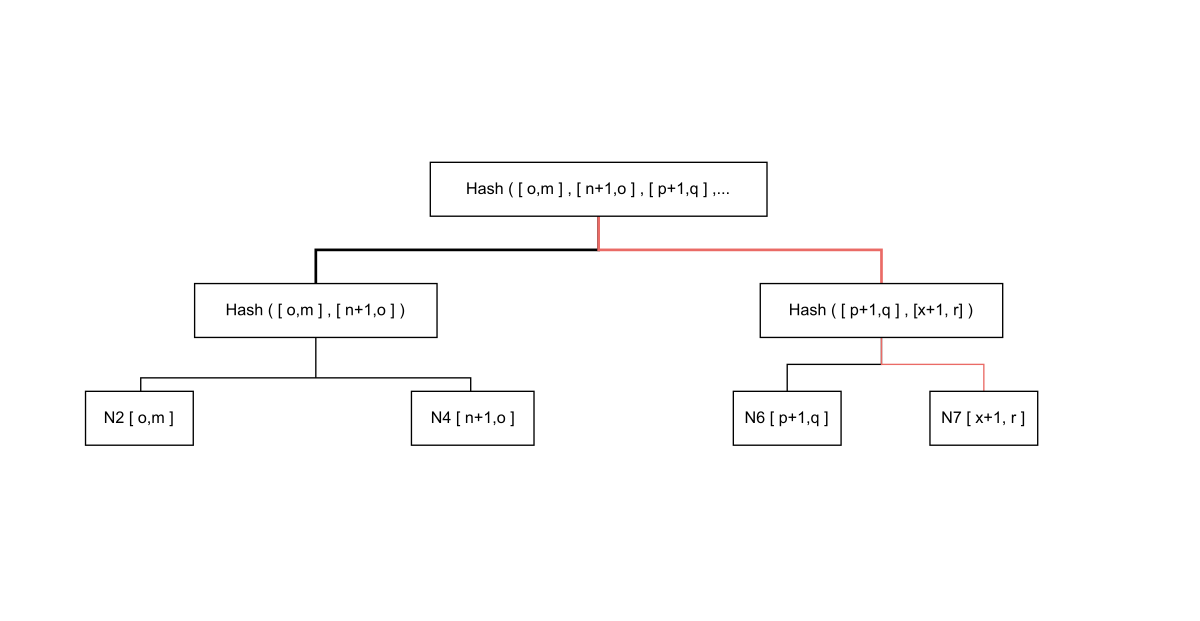
\includegraphics[width=\textwidth]{Images/chapter_10/section_5842597234343936/6153545749626880.png}
 \caption{The updated Merkle tree for Node B}
 \end{subfigure}
\end{figure}

The advantage of using Merkle trees is that each branch of the Merkle tree can be examined independently without requiring nodes to download the tree or the complete dataset. It reduces the quantity of data that must be exchanged for synchronization and the number of disc accesses that are required during the anti-entropy procedure.\\
\strut \\
The disadvantage is that when a node joins or departs the system, the tree's hashes are recalculated because multiple key ranges are affected.\\
\strut \\
We want our nodes to detect the failure of other nodes in the ring, so let's see how we can add it to our proposed design.\\
\\
Discuss the implications of scalability and fault tolerance when using consistent hashing in distributed key-value stores.\\
\strut \\

\subsection{Promote membership in the ring to detect failures}\label{D8V_cWDRynizFLCTbPeCo}
\\
The nodes can be offline for short periods, but they may also indefinitely go offline. We shouldn't rebalance partition assignments or fix unreachable replicas when a single node goes down because it's rarely a permanent departure. Therefore, the addition and removal of nodes from the ring should be done carefully.
\\
Planned commissioning and decommissioning of nodes results in membership changes. These changes form history. They're recorded persistently on the storage for each node and reconciled among the ring members using a gossip protocol. A \textbf{gossip-based protocol} also maintains an eventually consistent view of membership. When two nodes randomly choose one another as their peer, both nodes can efficiently synchronize their persisted membership histories.
\\
Let's learn how a gossip-based protocol works by considering the following example. Say node \protect\phantomsection\label{katex_inline_S13mWOR2eFyFLKmAanO2N}{{{\(\text{A}\)}}} starts up for the first time, and it randomly adds nodes \protect\phantomsection\label{katex_inline_pMnthC8F4XPbizayuwcf8}{{{\(\text{B}\)}}} and \protect\phantomsection\label{katex_inline_NgYT-vyVw1faYB5WEfBc5}{{{\(\text{E}\)}}} to its token set. The token set has virtual nodes in the consistent hash space and maps nodes to their respective token sets. This information is stored locally on the disk space of the node.
\\
Now, node \protect\phantomsection\label{katex_inline_Gt--C6KlJ90b1DI85RePc}{{{\(A\)}}} handles a request that results in a change, so it communicates this to \protect\phantomsection\label{katex_inline_vKaqsG92O9i8gPEX0ID5y}{{{\(\text{B}\)}}} and \protect\phantomsection\label{katex_inline_sU1P6G8auGo0OWV2wtZ01}{{{\(\text{E}\)}}}. Another node, \protect\phantomsection\label{katex_inline_2R8sV8HKp35CgmHx0YNAs}{{{\(\text{D}\)}}}, has \protect\phantomsection\label{katex_inline_kEmeHuaJaV9tcp8fNmrGx}{{{\(\text{C}\)}}} and \protect\phantomsection\label{katex_inline_SyzGgfR_SWsgP8mbigClw}{{{\(\text{E}\)}}} in its token set. It makes a change and tells \protect\phantomsection\label{katex_inline_fc1naNqSua2loNqOlfh6u}{{{\(\text{C}\)}}} and \protect\phantomsection\label{katex_inline_Z8Ul6WVnS5RA5EwYwVMQ0}{{{\(\text{E}\)}}}. The other nodes do the same process. This way, every node eventually knows about every other node's information. It 's an efficient way to share information asynchronously, and it doesn't take up a lot of bandwidth.

\begin{figure}[htbp]
 \centering
 \begin{subfigure}[b]{0.48\textwidth}
 \centering
 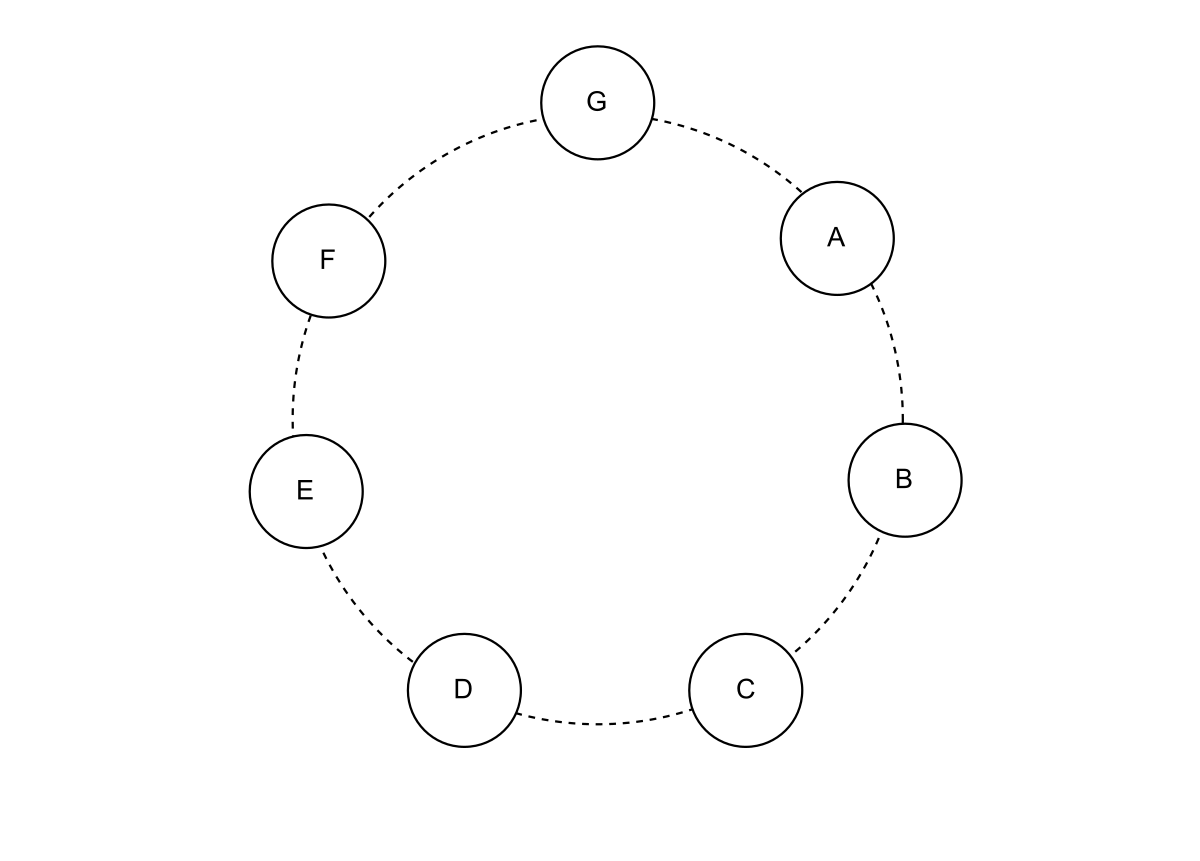
\includegraphics[width=\textwidth]{Images/chapter_10/section_5842597234343936/6682611825246208.png}
 \caption{A set of nodes in a ring}
 \end{subfigure}
 \hfill
 \begin{subfigure}[b]{0.48\textwidth}
 \centering
 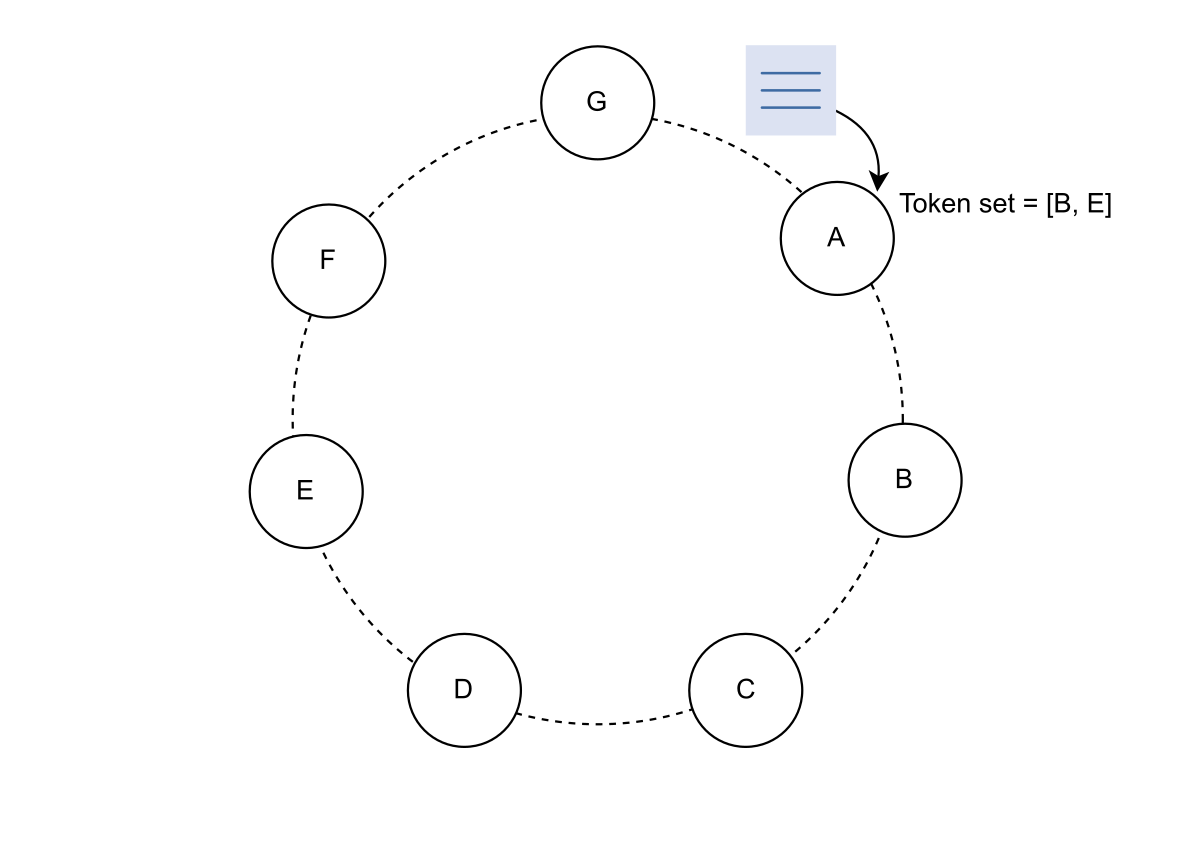
\includegraphics[width=\textwidth]{Images/chapter_10/section_5842597234343936/6665997347454976.png}
 \caption{Node A processes the request. Its token set has B and E in it}
 \end{subfigure}
\end{figure}

\begin{figure}[htbp]
 \centering
 \begin{subfigure}[b]{0.48\textwidth}
 \centering
 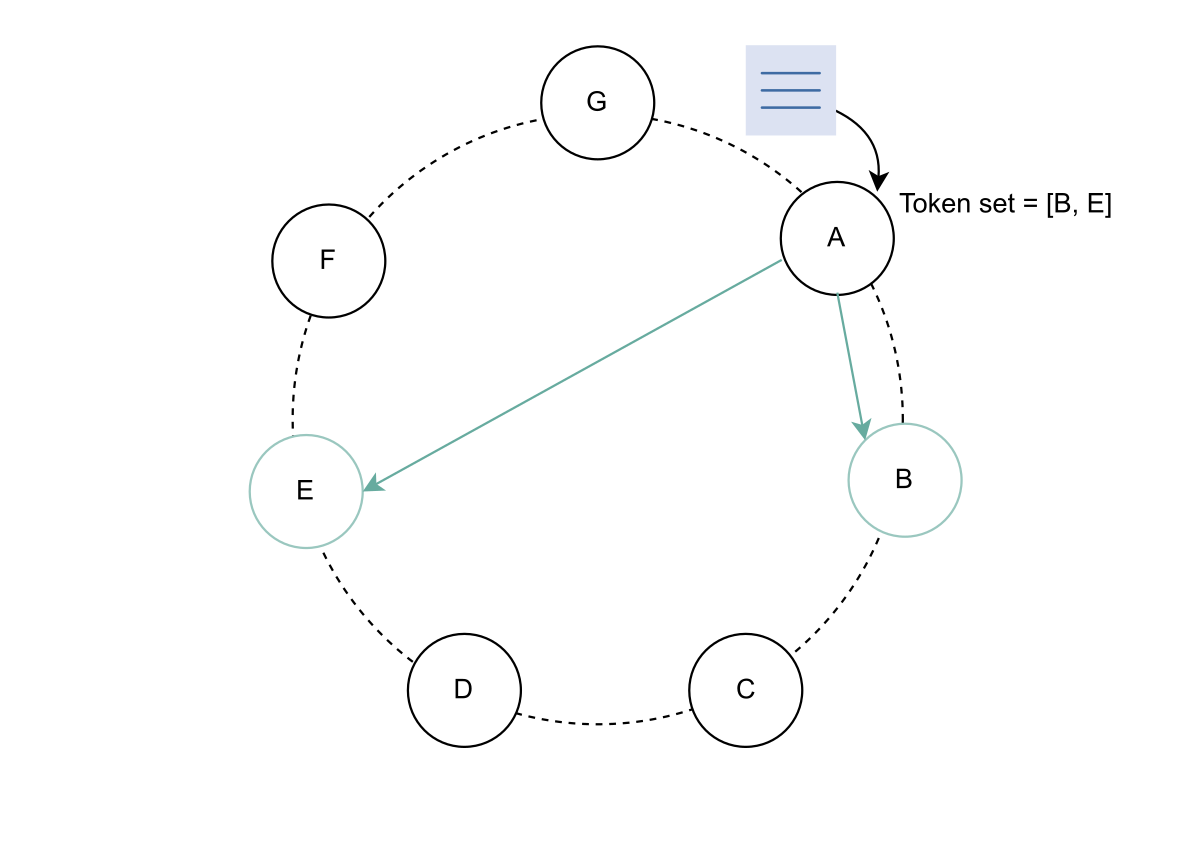
\includegraphics[width=\textwidth]{Images/chapter_10/section_5842597234343936/5685050238042112.png}
 \caption{Node A gossips membership information to Node B and E after few requests}
 \end{subfigure}
 \hfill
 \begin{subfigure}[b]{0.48\textwidth}
 \centering
 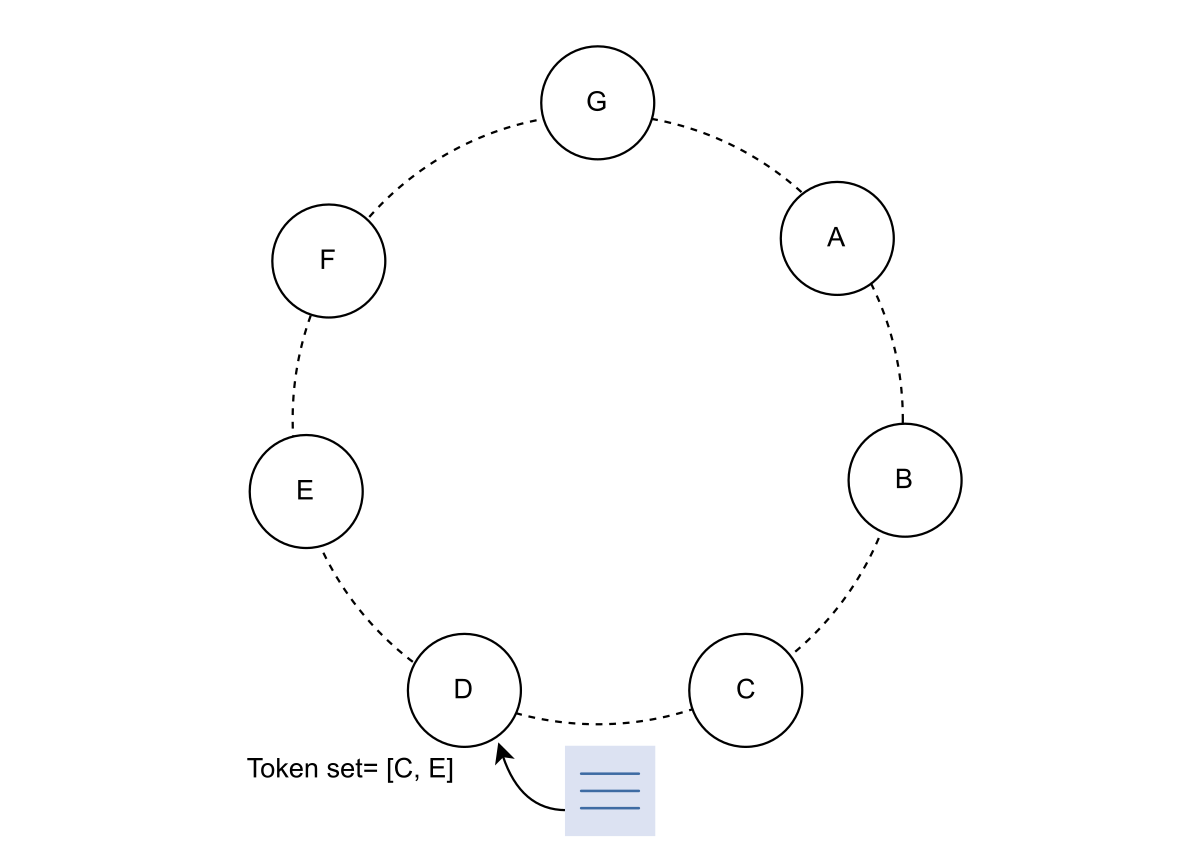
\includegraphics[width=\textwidth]{Images/chapter_10/section_5842597234343936/5872391879655424.png}
 \caption{Node D processes the request. Its token set has C and E in it}
 \end{subfigure}
\end{figure}

\begin{figure}[htbp]
 \centering
 \begin{subfigure}[b]{0.48\textwidth}
 \centering
 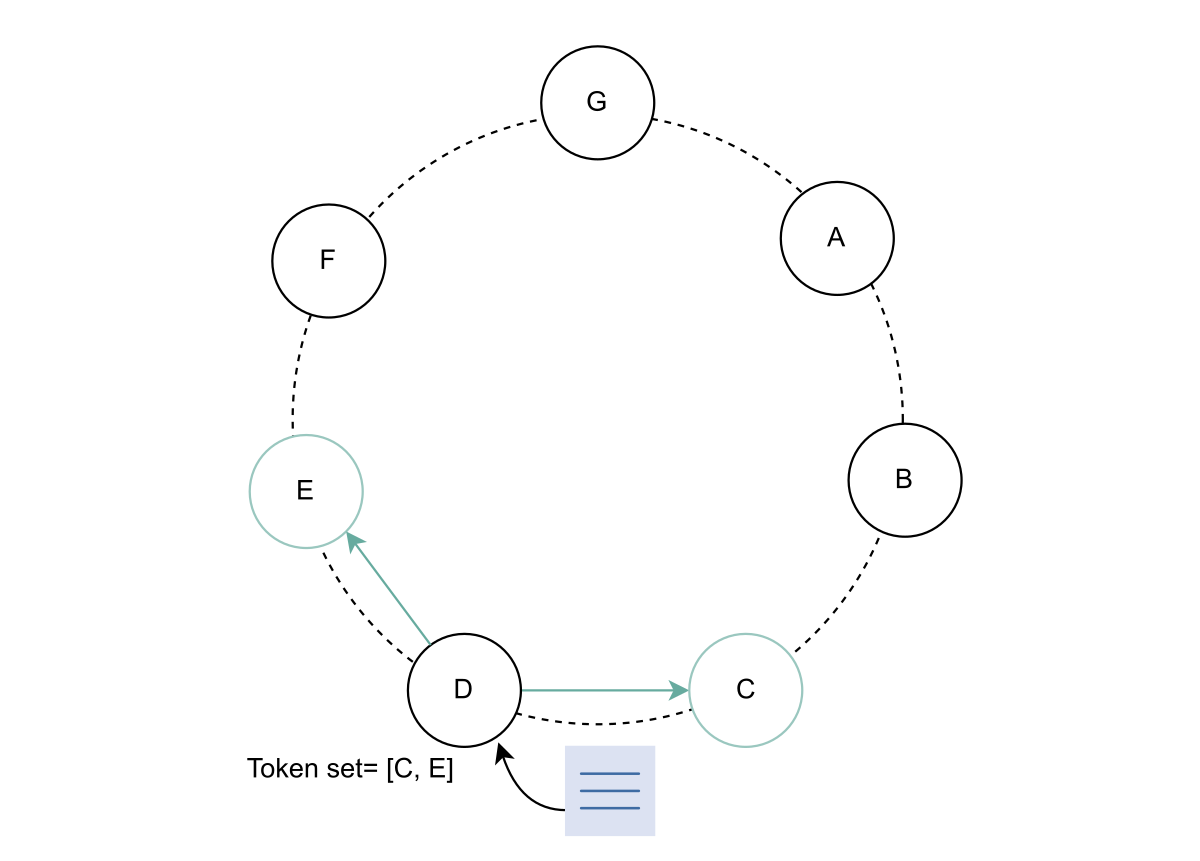
\includegraphics[width=\textwidth]{Images/chapter_10/section_5842597234343936/5599854125907968.png}
 \caption{Node D gossips membership information to Node C and E after a few requests}
 \end{subfigure}
\end{figure}

\subsection*{Test your knowledge!}
\vspace{0.3cm}
\noindent
\textbf{Question 1:} Can the gossip-based protocol fail in a system using consistent hashing, and if so, why?
\\[0.2cm]
\begin{itemize}
 \item No, the gossip-based protocol never fails as long as nodes are part of the consistent hashing ring.
 \item \textbf{[CORRECT]} Yes, it can fail if virtual nodes from the same physical server join the ring independently, causing logical partitioning and inconsistent updates.
\\[0.1cm]
\textit{Explanation:} 
The gossip-based protocol can fail when virtual nodes belonging to the same physical server (e.g., {{\(N1\)}} and {{\(N2\)}} of node {{\(A\)}}) both believe they are independent members of the ring. This leads to logical partitioning, where updates keep circulating within the same node. Additionally , issues like high churn or poor node connectivity can break the gossip network, preventing updates from propagating across all nodes.
 \item Yes, it can fail if the hash function used in consistent hashing produces duplicate keys.
 \item Yes, it can fail if the system uses a single physical node for all virtual nodes.
\end{itemize}
\vspace{0.3cm}
\noindent
\textbf{Question 2:} How can we prevent logical partitioning?
\\[0.2cm]
\begin{itemize}
 \item By assigning unique hash ranges to every virtual node without overlap.
 \item By periodically restarting all nodes to reset their membership states.
 \item \textbf{[CORRECT]} By designating a few nodes as seeds through a configuration service, allowing all nodes to reconcile membership via these known seeds.
\\[0.1cm]
\textit{Explanation:} 
To prevent logical partitioning, a few nodes are configured as seeds known to every node in the system. These seeds act as reference points that help all nodes reconcile their membership information, keeping the network connected and consistent.
 \item By disabling virtual nodes and using only physical nodes in the ring.
\end{itemize}

Decentralized failure detection protocols use a gossip-based protocol that allows each node to learn about the addition or removal of other nodes. The join and leave methods of the arriving or leaving nodes explicitly notify the other nodes about the permanent node additions and removals. The individual nodes detect temporary node failures when they fail to communicate with another node. If a node fails to communicate to any of the nodes present in its token set for the authorized time, then it communicates to the administrators that the node is dead.

\subsection{Conclusion}\label{78TR2aZpIPaW2Mm5ZSHga}
\\
A key-value store provides flexibility and allows us to scale the applications that have unstructured data. Web applications can use key-value stores to store information about a user's session and preferences. When using a user key, all the data is accessible, and key-value stores are ideal for rapid reads and write operations. Key -value stores can be used to power real-time recommendations and advertising because the stores can swiftly access and present fresh recommendations.

% End of section content